\chapter{O Método dos Elementos Finitos}

\begin{quote}
    "As far as the laws of mathematics refer to reality, they are not certain; and as far as they are certain, they do not refer to reality." (Albert Einstein)
\end{quote}

O Método dos Elementos Finitos (MEF), \emph{Finite Element Method} (FEM), é um método numérico, e tem como finalidade aproximar a solução de funções de campo numericamente, o domínios que são difíceis de se obter repostas diretas algebricamente. Para tanto, esse domínio é discretizado em vários elementos, ou sub-domínios (ver Figura \ref{fig:dominio_triangulo}), de tamanho finito, cujos comportamentos já são conhecidos da aplicação de leis físicas. A função de campo desconhecida é aproximada em cada elemento por meio de funções interpoladoras polinomiais, calculadas sobre o valor de campo em cada nó, que são os pontos do domínio sobre os quais os elementos são construídos (o campo, portanto, passa a ser definido não mais pelo conjunto de valores do contínuo, mais sim por essas variáveis desconhecidas discretizadas). Para cada elemento, são definidas equações, por meio das quais eles se relacionam entre si e com o campo. Isso leva à formação de um grande sistema linear, que pode ser resolvido facilmente, e obter-se, dessa forma, a aproximação da função de campo. \cite{Onate} Em sua, o método de elementos finitos segue o seguinte procedimento:

\begin{enumerate}
    \item definição do domínio ($\Omega$), e das condições de contorno ($\partial\Omega$);
    \item discretização do domínio em uma malha formada por nós que constituem os elementos ($\Omega^{(e)}$);
    \item aplicação da equação de governo sobre cada elemento;
    \item assemblagem dessas equações em um único grande sistema linear global ($K^{(g)}$);
    \item resolução do sistema, encontrando os valores nodais do campo ($U^{(g)}$).
\end{enumerate}

\begin{figure}
	\centering
    \caption{Domínio discretizado em elementos triangulares.}
    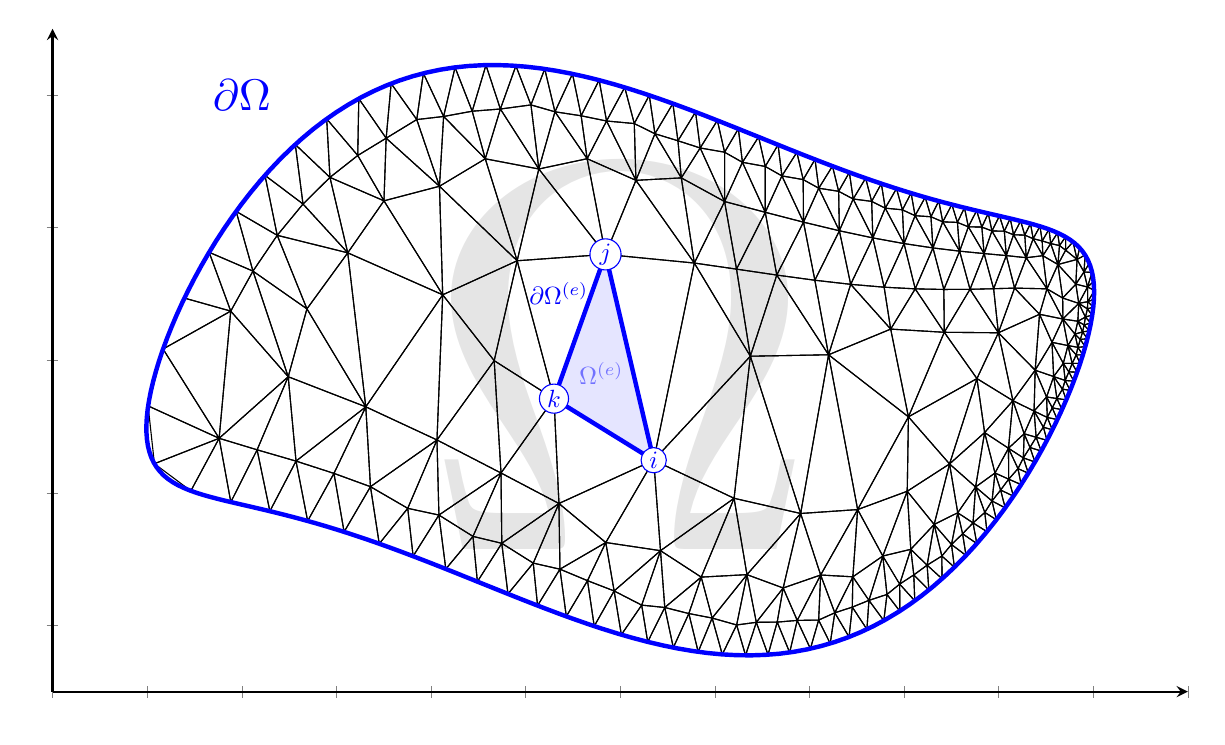
\begin{tikzpicture}
        \begin{axis}[
                xmin = -6, xmax = 6,
                ymin = -2.5, ymax = 2.5, 
                height = 10 cm, width = 16 cm,
                axis lines = left,
                xticklabels = {,,},
                yticklabels = {,,},
                axis line style = thick
            ]
                \draw (4.957784,0.2214301) -- (4.971856,0.2809534) -- (4.903003,0.2658061) -- cycle;\draw (4.971856,0.2809534) -- (4.985928,0.3404767) -- (4.917075,0.3253295) -- cycle;\draw (4.985928,0.3404767) -- (5.0,0.4) -- (4.93806,0.3872217) -- cycle;\draw (5.0,0.4) -- (5.010146,0.4615801) -- (4.94112,0.4413269) -- cycle;\draw (4.93717,0.162728) -- (4.957784,0.2214301) -- (4.886512,0.2134874) -- cycle;\draw (5.010146,0.4615801) -- (5.012756,0.5265611) -- (4.94112,0.4413269) -- cycle;\draw (5.012756,0.5265611) -- (5.004881,0.5938766) -- (4.938909,0.55204) -- cycle;\draw (4.889348,0.03979968) -- (4.914558,0.1022276) -- (4.837119,0.09719517) -- cycle;\draw (4.914558,0.1022276) -- (4.93717,0.162728) -- (4.863032,0.1559607) -- cycle;\draw (4.861032,-0.02440902) -- (4.889348,0.03979968) -- (4.819251,0.03970729) -- cycle;\draw (4.903003,0.2658061) -- (4.971856,0.2809534) -- (4.917075,0.3253295) -- cycle;\draw (4.903003,0.2658061) -- (4.917075,0.3253295) -- (4.836623,0.2940135) -- cycle;\draw (4.917075,0.3253295) -- (4.985928,0.3404767) -- (4.93806,0.3872217) -- cycle;\draw (4.917075,0.3253295) -- (4.846176,0.4289755) -- (4.836623,0.2940135) -- cycle;\draw (4.93806,0.3872217) -- (5.0,0.4) -- (4.94112,0.4413269) -- cycle;\draw (4.93806,0.3872217) -- (4.94112,0.4413269) -- (4.846176,0.4289755) -- cycle;\draw (4.957784,0.2214301) -- (4.903003,0.2658061) -- (4.886512,0.2134874) -- cycle;\draw (4.886512,0.2134874) -- (4.903003,0.2658061) -- (4.836623,0.2940135) -- cycle;\draw (5.004881,0.5938766) -- (4.986202,0.6620284) -- (4.938909,0.55204) -- cycle;\draw (4.93717,0.162728) -- (4.886512,0.2134874) -- (4.863032,0.1559607) -- cycle;\draw (4.863032,0.1559607) -- (4.886512,0.2134874) -- (4.805591,0.1969462) -- cycle;\draw (4.986202,0.6620284) -- (4.956748,0.7295127) -- (4.90139,0.6651808) -- cycle;\draw (4.829317,-0.09031633) -- (4.861032,-0.02440902) -- (4.776727,-0.02442582) -- cycle;\draw (4.914558,0.1022276) -- (4.863032,0.1559607) -- (4.837119,0.09719517) -- cycle;\draw (4.837119,0.09719517) -- (4.863032,0.1559607) -- (4.805591,0.1969462) -- cycle;\draw (4.956748,0.7295127) -- (4.913979,0.7931496) -- (4.90139,0.6651808) -- cycle;\draw (4.794248,-0.157996) -- (4.829317,-0.09031633) -- (4.741495,-0.087736) -- cycle;\draw (4.889348,0.03979968) -- (4.837119,0.09719517) -- (4.819251,0.03970729) -- cycle;\draw (4.819251,0.03970729) -- (4.837119,0.09719517) -- (4.732028,0.1103764) -- cycle;\draw (4.913979,0.7931496) -- (4.855867,0.8479657) -- (4.827994,0.7602062) -- cycle;\draw (4.755881,-0.2275484) -- (4.794248,-0.157996) -- (4.702832,-0.1529264) -- cycle;\draw (5.012756,0.5265611) -- (4.938909,0.55204) -- (4.94112,0.4413269) -- cycle;\draw (4.855867,0.8479657) -- (4.785727,0.8929289) -- (4.827994,0.7602062) -- cycle;\draw (4.714172,-0.2990376) -- (4.755881,-0.2275484) -- (4.673898,-0.21836) -- cycle;\draw (4.861032,-0.02440902) -- (4.819251,0.03970729) -- (4.776727,-0.02442582) -- cycle;\draw (4.776727,-0.02442582) -- (4.819251,0.03970729) -- (4.732028,0.1103764) -- cycle;\draw (4.986202,0.6620284) -- (4.90139,0.6651808) -- (4.938909,0.55204) -- cycle;\draw (4.829317,-0.09031633) -- (4.776727,-0.02442582) -- (4.741495,-0.087736) -- cycle;\draw (4.741495,-0.087736) -- (4.776727,-0.02442582) -- (4.682953,-0.02388099) -- cycle;\draw (4.785727,0.8929289) -- (4.707234,0.9300994) -- (4.707877,0.8299964) -- cycle;\draw (4.66901,-0.3724979) -- (4.714172,-0.2990376) -- (4.6153,-0.2888659) -- cycle;\draw (4.794248,-0.157996) -- (4.741495,-0.087736) -- (4.702832,-0.1529264) -- cycle;\draw (4.702832,-0.1529264) -- (4.741495,-0.087736) -- (4.682953,-0.02388099) -- cycle;\draw (4.620217,-0.4479242) -- (4.66901,-0.3724979) -- (4.566281,-0.3595372) -- cycle;\draw (4.707234,0.9300994) -- (4.622223,0.9611045) -- (4.642633,0.8645963) -- cycle;\draw (4.913979,0.7931496) -- (4.827994,0.7602062) -- (4.90139,0.6651808) -- cycle;\draw (4.755881,-0.2275484) -- (4.702832,-0.1529264) -- (4.673898,-0.21836) -- cycle;\draw (4.673898,-0.21836) -- (4.702832,-0.1529264) -- (4.581303,-0.1234217) -- cycle;\draw (4.56754,-0.525262) -- (4.620217,-0.4479242) -- (4.51356,-0.4318856) -- cycle;\draw (4.622223,0.9611045) -- (4.531635,0.9871874) -- (4.549841,0.8800674) -- cycle;\draw (4.846176,0.4289755) -- (4.94112,0.4413269) -- (4.938909,0.55204) -- cycle;\draw (4.93806,0.3872217) -- (4.846176,0.4289755) -- (4.917075,0.3253295) -- cycle;\draw (4.714172,-0.2990376) -- (4.673898,-0.21836) -- (4.6153,-0.2888659) -- cycle;\draw (4.6153,-0.2888659) -- (4.673898,-0.21836) -- (4.581303,-0.1234217) -- cycle;\draw (4.510708,-0.6044363) -- (4.56754,-0.525262) -- (4.472428,-0.5053484) -- cycle;\draw (4.805591,0.1969462) -- (4.886512,0.2134874) -- (4.836623,0.2940135) -- cycle;\draw (4.531635,0.9871874) -- (4.436162,1.010115) -- (4.460088,0.899499) -- cycle;\draw (4.66901,-0.3724979) -- (4.6153,-0.2888659) -- (4.566281,-0.3595372) -- cycle;\draw (4.566281,-0.3595372) -- (4.6153,-0.2888659) -- (4.506027,-0.2771593) -- cycle;\draw (4.449469,-0.6853741) -- (4.510708,-0.6044363) -- (4.396032,-0.5813056) -- cycle;\draw (4.707877,0.8299964) -- (4.707234,0.9300994) -- (4.642633,0.8645963) -- cycle;\draw (4.707877,0.8299964) -- (4.642633,0.8645963) -- (4.625992,0.7217137) -- cycle;\draw (4.785727,0.8929289) -- (4.707877,0.8299964) -- (4.827994,0.7602062) -- cycle;\draw (4.805591,0.1969462) -- (4.836623,0.2940135) -- (4.678231,0.310644) -- cycle;\draw (4.436162,1.010115) -- (4.336039,1.030872) -- (4.364544,0.9165118) -- cycle;\draw (4.620217,-0.4479242) -- (4.566281,-0.3595372) -- (4.51356,-0.4318856) -- cycle;\draw (4.51356,-0.4318856) -- (4.566281,-0.3595372) -- (4.506027,-0.2771593) -- cycle;\draw (4.383589,-0.7680124) -- (4.449469,-0.6853741) -- (4.330706,-0.6582747) -- cycle;\draw (4.732028,0.1103764) -- (4.837119,0.09719517) -- (4.805591,0.1969462) -- cycle;\draw (4.642633,0.8645963) -- (4.622223,0.9611045) -- (4.549841,0.8800674) -- cycle;\draw (4.642633,0.8645963) -- (4.549841,0.8800674) -- (4.625992,0.7217137) -- cycle;\draw (4.336039,1.030872) -- (4.23134,1.050217) -- (4.276047,0.9433966) -- cycle;\draw (4.56754,-0.525262) -- (4.51356,-0.4318856) -- (4.472428,-0.5053484) -- cycle;\draw (4.472428,-0.5053484) -- (4.51356,-0.4318856) -- (4.374301,-0.3838527) -- cycle;\draw (4.312867,-0.8523077) -- (4.383589,-0.7680124) -- (4.260684,-0.7367124) -- cycle;\draw (4.549841,0.8800674) -- (4.531635,0.9871874) -- (4.460088,0.899499) -- cycle;\draw (4.549841,0.8800674) -- (4.460088,0.899499) -- (4.467024,0.7882424) -- cycle;\draw (4.23134,1.050217) -- (4.122108,1.069087) -- (4.157126,0.9462107) -- cycle;\draw (4.510708,-0.6044363) -- (4.472428,-0.5053484) -- (4.396032,-0.5813056) -- cycle;\draw (4.396032,-0.5813056) -- (4.472428,-0.5053484) -- (4.374301,-0.3838527) -- cycle;\draw (4.460088,0.899499) -- (4.436162,1.010115) -- (4.364544,0.9165118) -- cycle;\draw (4.460088,0.899499) -- (4.364544,0.9165118) -- (4.467024,0.7882424) -- cycle;\draw (4.122108,1.069087) -- (4.008286,1.08806) -- (4.059354,0.9734298) -- cycle;\draw (4.237063,-0.938182) -- (4.312867,-0.8523077) -- (4.203966,-0.8177643) -- cycle;\draw (4.682953,-0.02388099) -- (4.776727,-0.02442582) -- (4.732028,0.1103764) -- cycle;\draw (4.836623,0.2940135) -- (4.846176,0.4289755) -- (4.678231,0.310644) -- cycle;\draw (4.449469,-0.6853741) -- (4.396032,-0.5813056) -- (4.330706,-0.6582747) -- cycle;\draw (4.330706,-0.6582747) -- (4.396032,-0.5813056) -- (4.269262,-0.5549482) -- cycle;\draw (4.364544,0.9165118) -- (4.336039,1.030872) -- (4.276047,0.9433966) -- cycle;\draw (4.364544,0.9165118) -- (4.276047,0.9433966) -- (4.291188,0.7731714) -- cycle;\draw (4.008286,1.08806) -- (3.889778,1.107575) -- (3.928765,0.9747425) -- cycle;\draw (4.155838,-1.02546) -- (4.237063,-0.938182) -- (4.105809,-0.8974663) -- cycle;\draw (4.938909,0.55204) -- (4.90139,0.6651808) -- (4.815769,0.5739968) -- cycle;\draw (4.90139,0.6651808) -- (4.827994,0.7602062) -- (4.815769,0.5739968) -- cycle;\draw (4.383589,-0.7680124) -- (4.330706,-0.6582747) -- (4.260684,-0.7367124) -- cycle;\draw (4.260684,-0.7367124) -- (4.330706,-0.6582747) -- (4.269262,-0.5549482) -- cycle;\draw (4.068821,-1.113913) -- (4.155838,-1.02546) -- (4.020468,-0.9793161) -- cycle;\draw (4.732028,0.1103764) -- (4.805591,0.1969462) -- (4.678231,0.310644) -- cycle;\draw (4.276047,0.9433966) -- (4.23134,1.050217) -- (4.157126,0.9462107) -- cycle;\draw (4.276047,0.9433966) -- (4.157126,0.9462107) -- (4.291188,0.7731714) -- cycle;\draw (3.889778,1.107575) -- (3.766497,1.128176) -- (3.822041,1.004182) -- cycle;\draw (4.581303,-0.1234217) -- (4.702832,-0.1529264) -- (4.682953,-0.02388099) -- cycle;\draw (4.938909,0.55204) -- (4.815769,0.5739968) -- (4.846176,0.4289755) -- cycle;\draw (4.312867,-0.8523077) -- (4.260684,-0.7367124) -- (4.203966,-0.8177643) -- cycle;\draw (4.203966,-0.8177643) -- (4.260684,-0.7367124) -- (4.103407,-0.6641533) -- cycle;\draw (4.157126,0.9462107) -- (4.122108,1.069087) -- (4.059354,0.9734298) -- cycle;\draw (4.157126,0.9462107) -- (4.059354,0.9734298) -- (4.080484,0.7890485) -- cycle;\draw (3.766497,1.128176) -- (3.638338,1.150301) -- (3.67944,1.00614) -- cycle;\draw (3.975609,-1.203253) -- (4.068821,-1.113913) -- (3.929432,-1.061779) -- cycle;\draw (4.237063,-0.938182) -- (4.203966,-0.8177643) -- (4.105809,-0.8974663) -- cycle;\draw (4.105809,-0.8974663) -- (4.203966,-0.8177643) -- (4.103407,-0.6641533) -- cycle;\draw (4.059354,0.9734298) -- (4.008286,1.08806) -- (3.928765,0.9747425) -- cycle;\draw (4.059354,0.9734298) -- (3.928765,0.9747425) -- (4.080484,0.7890485) -- cycle;\draw (4.682953,-0.02388099) -- (4.732028,0.1103764) -- (4.563331,0.1348475) -- cycle;\draw (3.875775,-1.293127) -- (3.975609,-1.203253) -- (3.8531,-1.14833) -- cycle;\draw (3.638338,1.150301) -- (3.505171,1.174253) -- (3.563819,1.039388) -- cycle;\draw (4.506027,-0.2771593) -- (4.6153,-0.2888659) -- (4.581303,-0.1234217) -- cycle;\draw (4.707877,0.8299964) -- (4.625992,0.7217137) -- (4.827994,0.7602062) -- cycle;\draw (4.155838,-1.02546) -- (4.105809,-0.8974663) -- (4.020468,-0.9793161) -- cycle;\draw (4.020468,-0.9793161) -- (4.105809,-0.8974663) -- (3.961036,-0.8508227) -- cycle;\draw (3.768883,-1.383123) -- (3.875775,-1.293127) -- (3.728865,-1.227114) -- cycle;\draw (3.928765,0.9747425) -- (3.889778,1.107575) -- (3.822041,1.004182) -- cycle;\draw (3.928765,0.9747425) -- (3.822041,1.004182) -- (3.845722,0.8042761) -- cycle;\draw (3.505171,1.174253) -- (3.366875,1.20038) -- (3.40889,1.043691) -- cycle;\draw (4.068821,-1.113913) -- (4.020468,-0.9793161) -- (3.929432,-1.061779) -- cycle;\draw (3.929432,-1.061779) -- (4.020468,-0.9793161) -- (3.961036,-0.8508227) -- cycle;\draw (3.822041,1.004182) -- (3.766497,1.128176) -- (3.67944,1.00614) -- cycle;\draw (3.822041,1.004182) -- (3.67944,1.00614) -- (3.845722,0.8042761) -- cycle;\draw (3.654491,-1.47276) -- (3.768883,-1.383123) -- (3.618596,-1.30914) -- cycle;\draw (4.581303,-0.1234217) -- (4.682953,-0.02388099) -- (4.563331,0.1348475) -- cycle;\draw (3.366875,1.20038) -- (3.223329,1.229015) -- (3.284154,1.081993) -- cycle;\draw (4.374301,-0.3838527) -- (4.51356,-0.4318856) -- (4.506027,-0.2771593) -- cycle;\draw (4.549841,0.8800674) -- (4.467024,0.7882424) -- (4.625992,0.7217137) -- cycle;\draw (4.846176,0.4289755) -- (4.815769,0.5739968) -- (4.676193,0.4690327) -- cycle;\draw (3.975609,-1.203253) -- (3.929432,-1.061779) -- (3.8531,-1.14833) -- cycle;\draw (3.8531,-1.14833) -- (3.929432,-1.061779) -- (3.75582,-0.9563786) -- cycle;\draw (3.67944,1.00614) -- (3.638338,1.150301) -- (3.563819,1.039388) -- cycle;\draw (3.67944,1.00614) -- (3.563819,1.039388) -- (3.587257,0.8225571) -- cycle;\draw (3.532149,-1.561476) -- (3.654491,-1.47276) -- (3.501184,-1.390061) -- cycle;\draw (3.223329,1.229015) -- (3.074389,1.260372) -- (3.116293,1.090014) -- cycle;\draw (4.625992,0.7217137) -- (4.467024,0.7882424) -- (4.51049,0.5384912) -- cycle;\draw (3.875775,-1.293127) -- (3.8531,-1.14833) -- (3.728865,-1.227114) -- cycle;\draw (3.728865,-1.227114) -- (3.8531,-1.14833) -- (3.75582,-0.9563786) -- cycle;\draw (3.563819,1.039388) -- (3.505171,1.174253) -- (3.40889,1.043691) -- cycle;\draw (3.563819,1.039388) -- (3.40889,1.043691) -- (3.587257,0.8225571) -- cycle;\draw (3.074389,1.260372) -- (2.919909,1.294658) -- (2.982263,1.134339) -- cycle;\draw (3.401409,-1.648618) -- (3.532149,-1.561476) -- (3.39923,-1.477053) -- cycle;\draw (4.269262,-0.5549482) -- (4.396032,-0.5813056) -- (4.374301,-0.3838527) -- cycle;\draw (4.506027,-0.2771593) -- (4.581303,-0.1234217) -- (4.385417,-0.07539267) -- cycle;\draw (4.364544,0.9165118) -- (4.291188,0.7731714) -- (4.467024,0.7882424) -- cycle;\draw (3.768883,-1.383123) -- (3.728865,-1.227114) -- (3.618596,-1.30914) -- cycle;\draw (3.618596,-1.30914) -- (3.728865,-1.227114) -- (3.567166,-1.150704) -- cycle;\draw (3.261824,-1.733416) -- (3.401409,-1.648618) -- (3.243551,-1.546053) -- cycle;\draw (3.40889,1.043691) -- (3.366875,1.20038) -- (3.284154,1.081993) -- cycle;\draw (3.40889,1.043691) -- (3.284154,1.081993) -- (3.30538,0.8468676) -- cycle;\draw (2.919909,1.294658) -- (2.759738,1.332071) -- (2.800969,1.147021) -- cycle;\draw (3.654491,-1.47276) -- (3.618596,-1.30914) -- (3.501184,-1.390061) -- cycle;\draw (3.501184,-1.390061) -- (3.618596,-1.30914) -- (3.567166,-1.150704) -- cycle;\draw (3.112959,-1.814965) -- (3.261824,-1.733416) -- (3.1027,-1.619589) -- cycle;\draw (3.284154,1.081993) -- (3.223329,1.229015) -- (3.116293,1.090014) -- cycle;\draw (3.284154,1.081993) -- (3.116293,1.090014) -- (3.30538,0.8468676) -- cycle;\draw (2.759738,1.332071) -- (2.593705,1.372722) -- (2.657296,1.198061) -- cycle;\draw (4.563331,0.1348475) -- (4.732028,0.1103764) -- (4.678231,0.310644) -- cycle;\draw (4.103407,-0.6641533) -- (4.260684,-0.7367124) -- (4.269262,-0.5549482) -- cycle;\draw (4.374301,-0.3838527) -- (4.506027,-0.2771593) -- (4.385417,-0.07539267) -- cycle;\draw (4.676193,0.4690327) -- (4.815769,0.5739968) -- (4.625992,0.7217137) -- cycle;\draw (4.846176,0.4289755) -- (4.676193,0.4690327) -- (4.678231,0.310644) -- cycle;\draw (4.678231,0.310644) -- (4.676193,0.4690327) -- (4.51049,0.5384912) -- cycle;\draw (3.532149,-1.561476) -- (3.501184,-1.390061) -- (3.39923,-1.477053) -- cycle;\draw (3.39923,-1.477053) -- (3.501184,-1.390061) -- (3.317859,-1.239057) -- cycle;\draw (4.157126,0.9462107) -- (4.080484,0.7890485) -- (4.291188,0.7731714) -- cycle;\draw (3.116293,1.090014) -- (3.074389,1.260372) -- (2.982263,1.134339) -- cycle;\draw (3.116293,1.090014) -- (2.982263,1.134339) -- (2.999753,0.8796282) -- cycle;\draw (2.593705,1.372722) -- (2.42162,1.41667) -- (2.462021,1.215979) -- cycle;\draw (2.95442,-1.89224) -- (3.112959,-1.814965) -- (2.953437,-1.688953) -- cycle;\draw (4.51049,0.5384912) -- (4.676193,0.4690327) -- (4.625992,0.7217137) -- cycle;\draw (3.401409,-1.648618) -- (3.39923,-1.477053) -- (3.243551,-1.546053) -- cycle;\draw (3.243551,-1.546053) -- (3.39923,-1.477053) -- (3.317859,-1.239057) -- cycle;\draw (2.785922,-1.964202) -- (2.95442,-1.89224) -- (2.819501,-1.766782) -- cycle;\draw (2.982263,1.134339) -- (2.919909,1.294658) -- (2.800969,1.147021) -- cycle;\draw (2.982263,1.134339) -- (2.800969,1.147021) -- (2.999753,0.8796282) -- cycle;\draw (2.42162,1.41667) -- (2.243277,1.463944) -- (2.308249,1.274053) -- cycle;\draw (4.467024,0.7882424) -- (4.291188,0.7731714) -- (4.51049,0.5384912) -- cycle;\draw (4.815769,0.5739968) -- (4.827994,0.7602062) -- (4.625992,0.7217137) -- cycle;\draw (3.961036,-0.8508227) -- (4.105809,-0.8974663) -- (4.103407,-0.6641533) -- cycle;\draw (4.269262,-0.5549482) -- (4.374301,-0.3838527) -- (4.15044,-0.3053903) -- cycle;\draw (3.261824,-1.733416) -- (3.243551,-1.546053) -- (3.1027,-1.619589) -- cycle;\draw (3.1027,-1.619589) -- (3.243551,-1.546053) -- (3.071024,-1.426535) -- cycle;\draw (3.928765,0.9747425) -- (3.845722,0.8042761) -- (4.080484,0.7890485) -- cycle;\draw (2.800969,1.147021) -- (2.759738,1.332071) -- (2.657296,1.198061) -- cycle;\draw (2.800969,1.147021) -- (2.657296,1.198061) -- (2.670046,0.9225129) -- cycle;\draw (2.243277,1.463944) -- (2.058444,1.514491) -- (2.098366,1.297261) -- cycle;\draw (2.60726,-2.029719) -- (2.785922,-1.964202) -- (2.628548,-1.811413) -- cycle;\draw (3.112959,-1.814965) -- (3.1027,-1.619589) -- (2.953437,-1.688953) -- cycle;\draw (2.953437,-1.688953) -- (3.1027,-1.619589) -- (3.071024,-1.426535) -- cycle;\draw (2.058444,1.514491) -- (1.866856,1.568176) -- (1.933885,1.362274) -- cycle;\draw (2.418315,-2.087564) -- (2.60726,-2.029719) -- (2.452714,-1.862415) -- cycle;\draw (2.657296,1.198061) -- (2.593705,1.372722) -- (2.462021,1.215979) -- cycle;\draw (2.657296,1.198061) -- (2.462021,1.215979) -- (2.670046,0.9225129) -- cycle;\draw (4.385417,-0.07539267) -- (4.581303,-0.1234217) -- (4.563331,0.1348475) -- cycle;\draw (3.75582,-0.9563786) -- (3.929432,-1.061779) -- (3.961036,-0.8508227) -- cycle;\draw (4.103407,-0.6641533) -- (4.269262,-0.5549482) -- (4.15044,-0.3053903) -- cycle;\draw (2.95442,-1.89224) -- (2.953437,-1.688953) -- (2.819501,-1.766782) -- cycle;\draw (2.819501,-1.766782) -- (2.953437,-1.688953) -- (2.775179,-1.477101) -- cycle;\draw (2.219138,-2.136655) -- (2.418315,-2.087564) -- (2.267743,-1.905256) -- cycle;\draw (2.462021,1.215979) -- (2.42162,1.41667) -- (2.308249,1.274053) -- cycle;\draw (2.462021,1.215979) -- (2.308249,1.274053) -- (2.315961,0.9764125) -- cycle;\draw (3.67944,1.00614) -- (3.587257,0.8225571) -- (3.845722,0.8042761) -- cycle;\draw (1.866856,1.568176) -- (1.668221,1.624792) -- (1.70874,1.390193) -- cycle;\draw (4.563331,0.1348475) -- (4.678231,0.310644) -- (4.431681,0.3463405) -- cycle;\draw (4.291188,0.7731714) -- (4.080484,0.7890485) -- (4.167947,0.543702) -- cycle;\draw (2.785922,-1.964202) -- (2.819501,-1.766782) -- (2.628548,-1.811413) -- cycle;\draw (2.628548,-1.811413) -- (2.819501,-1.766782) -- (2.775179,-1.477101) -- cycle;\draw (1.668221,1.624792) -- (1.462204,1.684023) -- (1.532699,1.461488) -- cycle;\draw (2.009885,-2.175947) -- (2.219138,-2.136655) -- (2.097157,-1.96016) -- cycle;\draw (2.308249,1.274053) -- (2.243277,1.463944) -- (2.098366,1.297261) -- cycle;\draw (2.308249,1.274053) -- (2.098366,1.297261) -- (2.315961,0.9764125) -- cycle;\draw (3.567166,-1.150704) -- (3.728865,-1.227114) -- (3.75582,-0.9563786) -- cycle;\draw (3.961036,-0.8508227) -- (4.103407,-0.6641533) -- (3.851279,-0.5458424) -- cycle;\draw (2.60726,-2.029719) -- (2.628548,-1.811413) -- (2.452714,-1.862415) -- cycle;\draw (2.452714,-1.862415) -- (2.628548,-1.811413) -- (2.458618,-1.633848) -- cycle;\draw (1.790808,-2.204433) -- (2.009885,-2.175947) -- (1.870762,-1.96267) -- cycle;\draw (2.098366,1.297261) -- (2.058444,1.514491) -- (1.933885,1.362274) -- cycle;\draw (2.098366,1.297261) -- (1.933885,1.362274) -- (1.937016,1.041251) -- cycle;\draw (1.462204,1.684023) -- (1.248433,1.745428) -- (1.291548,1.492716) -- cycle;\draw (3.40889,1.043691) -- (3.30538,0.8468676) -- (3.587257,0.8225571) -- cycle;\draw (2.418315,-2.087564) -- (2.452714,-1.862415) -- (2.267743,-1.905256) -- cycle;\draw (2.267743,-1.905256) -- (2.452714,-1.862415) -- (2.458618,-1.633848) -- cycle;\draw (1.248433,1.745428) -- (1.026493,1.808434) -- (1.10284,1.56888) -- cycle;\draw (1.562265,-2.221443) -- (1.790808,-2.204433) -- (1.658871,-1.975588) -- cycle;\draw (1.933885,1.362274) -- (1.866856,1.568176) -- (1.70874,1.390193) -- cycle;\draw (1.933885,1.362274) -- (1.70874,1.390193) -- (1.937016,1.041251) -- cycle;\draw (4.080484,0.7890485) -- (3.845722,0.8042761) -- (3.946406,0.5392471) -- cycle;\draw (3.75582,-0.9563786) -- (3.961036,-0.8508227) -- (3.851279,-0.5458424) -- cycle;\draw (2.219138,-2.136655) -- (2.267743,-1.905256) -- (2.097157,-1.96016) -- cycle;\draw (2.097157,-1.96016) -- (2.267743,-1.905256) -- (2.118257,-1.620272) -- cycle;\draw (1.324648,-2.226458) -- (1.562265,-2.221443) -- (1.438248,-1.977175) -- cycle;\draw (3.317859,-1.239057) -- (3.501184,-1.390061) -- (3.567166,-1.150704) -- cycle;\draw (4.15044,-0.3053903) -- (4.374301,-0.3838527) -- (4.385417,-0.07539267) -- cycle;\draw (1.70874,1.390193) -- (1.668221,1.624792) -- (1.532699,1.461488) -- cycle;\draw (1.70874,1.390193) -- (1.532699,1.461488) -- (1.532781,1.115714) -- cycle;\draw (1.026493,1.808434) -- (0.7959219,1.87228) -- (0.8449012,1.6009) -- cycle;\draw (3.116293,1.090014) -- (2.999753,0.8796282) -- (3.30538,0.8468676) -- cycle;\draw (2.009885,-2.175947) -- (2.097157,-1.96016) -- (1.870762,-1.96267) -- cycle;\draw (1.870762,-1.96267) -- (2.097157,-1.96016) -- (2.118257,-1.620272) -- cycle;\draw (0.7959219,1.87228) -- (0.5562157,1.935994) -- (0.6098994,1.655193) -- cycle;\draw (1.078342,-2.219175) -- (1.324648,-2.226458) -- (1.230389,-1.997044) -- cycle;\draw (1.532699,1.461488) -- (1.462204,1.684023) -- (1.291548,1.492716) -- cycle;\draw (1.532699,1.461488) -- (1.291548,1.492716) -- (1.532781,1.115714) -- cycle;\draw (4.431681,0.3463405) -- (4.678231,0.310644) -- (4.51049,0.5384912) -- cycle;\draw (4.431681,0.3463405) -- (4.51049,0.5384912) -- (4.167947,0.543702) -- cycle;\draw (4.563331,0.1348475) -- (4.431681,0.3463405) -- (4.385417,-0.07539267) -- cycle;\draw (3.567166,-1.150704) -- (3.75582,-0.9563786) -- (3.480671,-0.7824747) -- cycle;\draw (0.8236913,-2.199606) -- (1.078342,-2.219175) -- (0.9713398,-1.944926) -- cycle;\draw (1.790808,-2.204433) -- (1.870762,-1.96267) -- (1.658871,-1.975588) -- cycle;\draw (1.658871,-1.975588) -- (1.870762,-1.96267) -- (1.72204,-1.71823) -- cycle;\draw (0.5562157,1.935994) -- (0.3068405,1.998364) -- (0.3667546,1.708193) -- cycle;\draw (3.071024,-1.426535) -- (3.243551,-1.546053) -- (3.317859,-1.239057) -- cycle;\draw (1.291548,1.492716) -- (1.248433,1.745428) -- (1.10284,1.56888) -- cycle;\draw (1.291548,1.492716) -- (1.10284,1.56888) -- (1.102826,1.196921) -- cycle;\draw (2.800969,1.147021) -- (2.670046,0.9225129) -- (2.999753,0.8796282) -- cycle;\draw (3.845722,0.8042761) -- (3.587257,0.8225571) -- (3.696782,0.5347843) -- cycle;\draw (4.167947,0.543702) -- (4.080484,0.7890485) -- (3.946406,0.5392471) -- cycle;\draw (4.167947,0.543702) -- (3.946406,0.5392471) -- (3.996703,0.2069171) -- cycle;\draw (4.291188,0.7731714) -- (4.167947,0.543702) -- (4.51049,0.5384912) -- cycle;\draw (1.562265,-2.221443) -- (1.658871,-1.975588) -- (1.438248,-1.977175) -- cycle;\draw (1.438248,-1.977175) -- (1.658871,-1.975588) -- (1.72204,-1.71823) -- cycle;\draw (0.3068405,1.998364) -- (0.04723287,2.05782) -- (0.1483761,1.785116) -- cycle;\draw (0.5609525,-2.167965) -- (0.8236913,-2.199606) -- (0.7251818,-1.910921) -- cycle;\draw (1.10284,1.56888) -- (1.026493,1.808434) -- (0.8449012,1.6009) -- cycle;\draw (1.10284,1.56888) -- (0.8449012,1.6009) -- (1.102826,1.196921) -- cycle;\draw (3.317859,-1.239057) -- (3.567166,-1.150704) -- (3.480671,-0.7824747) -- cycle;\draw (0.2902728,-2.124676) -- (0.5609525,-2.167965) -- (0.4705707,-1.865209) -- cycle;\draw (1.324648,-2.226458) -- (1.438248,-1.977175) -- (1.230389,-1.997044) -- cycle;\draw (1.230389,-1.997044) -- (1.438248,-1.977175) -- (1.339368,-1.617484) -- cycle;\draw (0.04723287,2.05782) -- (-0.223152,2.112443) -- (-0.1446873,1.804327) -- cycle;\draw (0.8449012,1.6009) -- (0.7959219,1.87228) -- (0.6098994,1.655193) -- cycle;\draw (0.8449012,1.6009) -- (0.6098994,1.655193) -- (0.6454989,1.375159) -- cycle;\draw (2.775179,-1.477101) -- (2.953437,-1.688953) -- (3.071024,-1.426535) -- cycle;\draw (3.851279,-0.5458424) -- (4.103407,-0.6641533) -- (4.15044,-0.3053903) -- cycle;\draw (2.462021,1.215979) -- (2.315961,0.9764125) -- (2.670046,0.9225129) -- cycle;\draw (3.587257,0.8225571) -- (3.30538,0.8468676) -- (3.420344,0.5335478) -- cycle;\draw (3.946406,0.5392471) -- (3.845722,0.8042761) -- (3.696782,0.5347843) -- cycle;\draw (3.946406,0.5392471) -- (3.696782,0.5347843) -- (3.996703,0.2069171) -- cycle;\draw (0.01166126,-2.070405) -- (0.2902728,-2.124676) -- (0.2266713,-1.847469) -- cycle;\draw (1.078342,-2.219175) -- (1.230389,-1.997044) -- (0.9713398,-1.944926) -- cycle;\draw (0.9713398,-1.944926) -- (1.230389,-1.997044) -- (1.339368,-1.617484) -- cycle;\draw (-0.223152,2.112443) -- (-0.5048027,2.159827) -- (-0.4131879,1.84363) -- cycle;\draw (0.6098994,1.655193) -- (0.5562157,1.935994) -- (0.3667546,1.708193) -- cycle;\draw (0.6098994,1.655193) -- (0.3667546,1.708193) -- (0.6454989,1.375159) -- cycle;\draw (3.071024,-1.426535) -- (3.317859,-1.239057) -- (3.03342,-0.9884558) -- cycle;\draw (-0.5048027,2.159827) -- (-0.7980679,2.197007) -- (-0.6900482,1.87385) -- cycle;\draw (-0.2750093,-2.005977) -- (0.01166126,-2.070405) -- (-0.06476378,-1.740473) -- cycle;\draw (0.8236913,-2.199606) -- (0.9713398,-1.944926) -- (0.7251818,-1.910921) -- cycle;\draw (0.7251818,-1.910921) -- (0.9713398,-1.944926) -- (0.8558776,-1.636119) -- cycle;\draw (2.458618,-1.633848) -- (2.628548,-1.811413) -- (2.775179,-1.477101) -- cycle;\draw (0.3667546,1.708193) -- (0.3068405,1.998364) -- (0.1483761,1.785116) -- cycle;\draw (0.3667546,1.708193) -- (0.1483761,1.785116) -- (0.16574,1.356876) -- cycle;\draw (-0.5700138,-1.932418) -- (-0.2750093,-2.005977) -- (-0.3461177,-1.662825) -- cycle;\draw (2.098366,1.297261) -- (1.937016,1.041251) -- (2.315961,0.9764125) -- cycle;\draw (-0.7980679,2.197007) -- (-1.103023,2.220447) -- (-0.9437152,1.925671) -- cycle;\draw (0.5609525,-2.167965) -- (0.7251818,-1.910921) -- (0.4705707,-1.865209) -- cycle;\draw (0.4705707,-1.865209) -- (0.7251818,-1.910921) -- (0.8558776,-1.636119) -- cycle;\draw (2.775179,-1.477101) -- (3.071024,-1.426535) -- (3.03342,-0.9884558) -- cycle;\draw (0.1483761,1.785116) -- (0.04723287,2.05782) -- (-0.1446873,1.804327) -- cycle;\draw (0.1483761,1.785116) -- (-0.1446873,1.804327) -- (0.16574,1.356876) -- cycle;\draw (3.30538,0.8468676) -- (2.999753,0.8796282) -- (3.117725,0.5382074) -- cycle;\draw (3.696782,0.5347843) -- (3.587257,0.8225571) -- (3.420344,0.5335478) -- cycle;\draw (3.696782,0.5347843) -- (3.420344,0.5335478) -- (3.424796,0.2106327) -- cycle;\draw (-0.8737736,-1.850959) -- (-0.5700138,-1.932418) -- (-0.6372948,-1.576222) -- cycle;\draw (0.2902728,-2.124676) -- (0.4705707,-1.865209) -- (0.2266713,-1.847469) -- cycle;\draw (0.2266713,-1.847469) -- (0.4705707,-1.865209) -- (0.4256156,-1.436581) -- cycle;\draw (-1.103023,2.220447) -- (-1.419308,2.225934) -- (-1.266864,1.894717) -- cycle;\draw (-0.1446873,1.804327) -- (-0.223152,2.112443) -- (-0.4131879,1.84363) -- cycle;\draw (-0.1446873,1.804327) -- (-0.4131879,1.84363) -- (-0.3497612,1.519874) -- cycle;\draw (2.118257,-1.620272) -- (2.267743,-1.905256) -- (2.458618,-1.633848) -- cycle;\draw (-1.186842,-1.76302) -- (-0.8737736,-1.850959) -- (-0.9195799,-1.530421) -- cycle;\draw (1.70874,1.390193) -- (1.532781,1.115714) -- (1.937016,1.041251) -- cycle;\draw (3.480671,-0.7824747) -- (3.75582,-0.9563786) -- (3.851279,-0.5458424) -- cycle;\draw (2.458618,-1.633848) -- (2.775179,-1.477101) -- (2.509265,-1.126632) -- cycle;\draw (-1.419308,2.225934) -- (-1.745899,2.208776) -- (-1.564785,1.878178) -- cycle;\draw (0.01166126,-2.070405) -- (0.2266713,-1.847469) -- (-0.06476378,-1.740473) -- cycle;\draw (-0.06476378,-1.740473) -- (0.2266713,-1.847469) -- (0.4256156,-1.436581) -- cycle;\draw (4.15044,-0.3053903) -- (4.385417,-0.07539267) -- (3.996703,0.2069171) -- cycle;\draw (4.431681,0.3463405) -- (4.167947,0.543702) -- (3.996703,0.2069171) -- cycle;\draw (-0.4131879,1.84363) -- (-0.5048027,2.159827) -- (-0.6900482,1.87385) -- cycle;\draw (-0.4131879,1.84363) -- (-0.6900482,1.87385) -- (-0.3497612,1.519874) -- cycle;\draw (-1.509905,-1.670291) -- (-1.186842,-1.76302) -- (-1.252071,-1.381142) -- cycle;\draw (2.999753,0.8796282) -- (2.670046,0.9225129) -- (2.789334,0.5507515) -- cycle;\draw (3.420344,0.5335478) -- (3.30538,0.8468676) -- (3.117725,0.5382074) -- cycle;\draw (3.420344,0.5335478) -- (3.117725,0.5382074) -- (3.424796,0.2106327) -- cycle;\draw (-1.745899,2.208776) -- (-2.080892,2.163962) -- (-1.866855,1.838467) -- cycle;\draw (-0.2750093,-2.005977) -- (-0.06476378,-1.740473) -- (-0.3461177,-1.662825) -- cycle;\draw (-0.3461177,-1.662825) -- (-0.06476378,-1.740473) -- (-0.1527942,-1.375203) -- cycle;\draw (-0.6900482,1.87385) -- (-0.7980679,2.197007) -- (-0.9437152,1.925671) -- cycle;\draw (-0.6900482,1.87385) -- (-0.9437152,1.925671) -- (-0.8605728,1.442333) -- cycle;\draw (-1.843752,-1.574721) -- (-1.509905,-1.670291) -- (-1.556525,-1.328974) -- cycle;\draw (1.72204,-1.71823) -- (1.870762,-1.96267) -- (2.118257,-1.620272) -- cycle;\draw (2.118257,-1.620272) -- (2.458618,-1.633848) -- (2.509265,-1.126632) -- cycle;\draw (-2.080892,2.163962) -- (-2.421384,2.086734) -- (-2.150831,1.81516) -- cycle;\draw (1.291548,1.492716) -- (1.102826,1.196921) -- (1.532781,1.115714) -- cycle;\draw (-0.5700138,-1.932418) -- (-0.3461177,-1.662825) -- (-0.6372948,-1.576222) -- cycle;\draw (-0.6372948,-1.576222) -- (-0.3461177,-1.662825) -- (-0.1527942,-1.375203) -- cycle;\draw (-0.9437152,1.925671) -- (-1.103023,2.220447) -- (-1.266864,1.894717) -- cycle;\draw (-0.9437152,1.925671) -- (-1.266864,1.894717) -- (-0.8605728,1.442333) -- cycle;\draw (2.670046,0.9225129) -- (2.315961,0.9764125) -- (2.435598,0.5723432) -- cycle;\draw (-2.189247,-1.47857) -- (-1.843752,-1.574721) -- (-1.916643,-1.167836) -- cycle;\draw (-2.421384,2.086734) -- (-2.763501,1.973007) -- (-2.474333,1.674569) -- cycle;\draw (3.117725,0.5382074) -- (2.999753,0.8796282) -- (2.789334,0.5507515) -- cycle;\draw (3.117725,0.5382074) -- (2.789334,0.5507515) -- (2.858475,0.2345827) -- cycle;\draw (-0.8737736,-1.850959) -- (-0.6372948,-1.576222) -- (-0.9195799,-1.530421) -- cycle;\draw (-0.9195799,-1.530421) -- (-0.6372948,-1.576222) -- (-0.6479176,-1.080763) -- cycle;\draw (-1.266864,1.894717) -- (-1.419308,2.225934) -- (-1.564785,1.878178) -- cycle;\draw (-1.266864,1.894717) -- (-1.564785,1.878178) -- (-1.42658,1.5193) -- cycle;\draw (-2.763501,1.973007) -- (-3.10281,1.820201) -- (-2.77446,1.544219) -- cycle;\draw (-2.547275,-1.384405) -- (-2.189247,-1.47857) -- (-2.246037,-1.117272) -- cycle;\draw (1.339368,-1.617484) -- (1.438248,-1.977175) -- (1.72204,-1.71823) -- cycle;\draw (-1.186842,-1.76302) -- (-0.9195799,-1.530421) -- (-1.252071,-1.381142) -- cycle;\draw (-1.252071,-1.381142) -- (-0.9195799,-1.530421) -- (-0.6479176,-1.080763) -- cycle;\draw (1.72204,-1.71823) -- (2.118257,-1.620272) -- (1.906732,-1.156191) -- cycle;\draw (0.8449012,1.6009) -- (0.6454989,1.375159) -- (1.102826,1.196921) -- cycle;\draw (3.03342,-0.9884558) -- (3.317859,-1.239057) -- (3.480671,-0.7824747) -- cycle;\draw (-1.564785,1.878178) -- (-1.745899,2.208776) -- (-1.866855,1.838467) -- cycle;\draw (-1.564785,1.878178) -- (-1.866855,1.838467) -- (-1.42658,1.5193) -- cycle;\draw (-3.10281,1.820201) -- (-3.434709,1.627173) -- (-3.068293,1.378997) -- cycle;\draw (-2.918641,-1.294954) -- (-2.547275,-1.384405) -- (-2.640059,-0.9540017) -- cycle;\draw (3.851279,-0.5458424) -- (4.15044,-0.3053903) -- (3.770158,-0.1385871) -- cycle;\draw (2.315961,0.9764125) -- (1.937016,1.041251) -- (2.057079,0.60317) -- cycle;\draw (-1.509905,-1.670291) -- (-1.252071,-1.381142) -- (-1.556525,-1.328974) -- cycle;\draw (-1.556525,-1.328974) -- (-1.252071,-1.381142) -- (-1.260254,-0.8508811) -- cycle;\draw (2.789334,0.5507515) -- (2.670046,0.9225129) -- (2.435598,0.5723432) -- cycle;\draw (2.789334,0.5507515) -- (2.435598,0.5723432) -- (2.858475,0.2345827) -- cycle;\draw (-1.866855,1.838467) -- (-2.080892,2.163962) -- (-2.150831,1.81516) -- cycle;\draw (-1.866855,1.838467) -- (-2.150831,1.81516) -- (-1.910694,1.312065) -- cycle;\draw (-3.434709,1.627173) -- (-3.754975,1.394323) -- (-3.353019,1.178139) -- cycle;\draw (-3.303933,-1.21274) -- (-2.918641,-1.294954) -- (-3.025905,-0.8537066) -- cycle;\draw (4.431681,0.3463405) -- (3.996703,0.2069171) -- (4.385417,-0.07539267) -- cycle;\draw (-1.843752,-1.574721) -- (-1.556525,-1.328974) -- (-1.916643,-1.167836) -- cycle;\draw (-1.916643,-1.167836) -- (-1.556525,-1.328974) -- (-1.260254,-0.8508811) -- cycle;\draw (0.8558776,-1.636119) -- (0.9713398,-1.944926) -- (1.339368,-1.617484) -- cycle;\draw (-2.150831,1.81516) -- (-2.421384,2.086734) -- (-2.474333,1.674569) -- cycle;\draw (-2.150831,1.81516) -- (-2.474333,1.674569) -- (-1.910694,1.312065) -- cycle;\draw (-3.754975,1.394323) -- (-4.0598,1.122874) -- (-3.625477,0.9420269) -- cycle;\draw (-3.70331,-1.138966) -- (-3.303933,-1.21274) -- (-3.427004,-0.7610851) -- cycle;\draw (0.3667546,1.708193) -- (0.16574,1.356876) -- (0.6454989,1.375159) -- cycle;\draw (1.339368,-1.617484) -- (1.72204,-1.71823) -- (1.906732,-1.156191) -- cycle;\draw (1.937016,1.041251) -- (1.532781,1.115714) -- (1.654533,0.6422065) -- cycle;\draw (-2.189247,-1.47857) -- (-1.916643,-1.167836) -- (-2.246037,-1.117272) -- cycle;\draw (-2.246037,-1.117272) -- (-1.916643,-1.167836) -- (-1.936959,-0.6015458) -- cycle;\draw (-2.474333,1.674569) -- (-2.763501,1.973007) -- (-2.77446,1.544219) -- cycle;\draw (-2.474333,1.674569) -- (-2.77446,1.544219) -- (-2.497419,1.202192) -- cycle;\draw (3.770158,-0.1385871) -- (4.15044,-0.3053903) -- (3.996703,0.2069171) -- cycle;\draw (3.851279,-0.5458424) -- (3.770158,-0.1385871) -- (3.480671,-0.7824747) -- cycle;\draw (-4.116085,-1.070089) -- (-3.70331,-1.138966) -- (-3.838166,-0.6758455) -- cycle;\draw (-4.0598,1.122874) -- (-4.345333,0.8141347) -- (-3.881929,0.6719672) -- cycle;\draw (2.435598,0.5723432) -- (2.315961,0.9764125) -- (2.057079,0.60317) -- cycle;\draw (2.435598,0.5723432) -- (2.057079,0.60317) -- (2.20181,0.04099137) -- cycle;\draw (3.696782,0.5347843) -- (3.424796,0.2106327) -- (3.996703,0.2069171) -- cycle;\draw (-2.547275,-1.384405) -- (-2.246037,-1.117272) -- (-2.640059,-0.9540017) -- cycle;\draw (-2.640059,-0.9540017) -- (-2.246037,-1.117272) -- (-1.936959,-0.6015458) -- cycle;\draw (-4.538534,-0.9854896) -- (-4.116085,-1.070089) -- (-4.239449,-0.5890606) -- cycle;\draw (0.4256156,-1.436581) -- (0.4705707,-1.865209) -- (0.8558776,-1.636119) -- cycle;\draw (-2.77446,1.544219) -- (-3.10281,1.820201) -- (-3.068293,1.378997) -- cycle;\draw (-2.77446,1.544219) -- (-3.068293,1.378997) -- (-2.497419,1.202192) -- cycle;\draw (-4.345333,0.8141347) -- (-4.606348,0.4686135) -- (-4.117004,0.3703004) -- cycle;\draw (-4.923608,-0.7807422) -- (-4.538534,-0.9854896) -- (-4.239449,-0.5890606) -- cycle;\draw (-0.1446873,1.804327) -- (-0.3497612,1.519874) -- (0.16574,1.356876) -- cycle;\draw (1.532781,1.115714) -- (1.102826,1.196921) -- (1.229147,0.6869177) -- cycle;\draw (2.509265,-1.126632) -- (2.775179,-1.477101) -- (3.03342,-0.9884558) -- cycle;\draw (-2.918641,-1.294954) -- (-2.640059,-0.9540017) -- (-3.025905,-0.8537066) -- cycle;\draw (-3.025905,-0.8537066) -- (-2.640059,-0.9540017) -- (-2.689459,-0.3517044) -- cycle;\draw (-4.990237,-0.3447668) -- (-4.923608,-0.7807422) -- (-4.239449,-0.5890606) -- cycle;\draw (-3.068293,1.378997) -- (-3.434709,1.627173) -- (-3.353019,1.178139) -- cycle;\draw (-3.068293,1.378997) -- (-3.353019,1.178139) -- (-2.880107,0.8099991) -- cycle;\draw (0.8558776,-1.636119) -- (1.339368,-1.617484) -- (1.20319,-1.041589) -- cycle;\draw (-4.606348,0.4686135) -- (-4.832226,0.08454963) -- (-4.117004,0.3703004) -- cycle;\draw (3.770158,-0.1385871) -- (3.996703,0.2069171) -- (3.424796,0.2106327) -- cycle;\draw (3.770158,-0.1385871) -- (3.046024,-0.4272705) -- (3.480671,-0.7824747) -- cycle;\draw (2.057079,0.60317) -- (1.937016,1.041251) -- (1.654533,0.6422065) -- cycle;\draw (2.057079,0.60317) -- (1.654533,0.6422065) -- (2.20181,0.04099137) -- cycle;\draw (-3.303933,-1.21274) -- (-3.025905,-0.8537066) -- (-3.427004,-0.7610851) -- cycle;\draw (-3.427004,-0.7610851) -- (-3.025905,-0.8537066) -- (-2.689459,-0.3517044) -- cycle;\draw (-3.353019,1.178139) -- (-3.754975,1.394323) -- (-3.625477,0.9420269) -- cycle;\draw (-3.353019,1.178139) -- (-3.625477,0.9420269) -- (-2.880107,0.8099991) -- cycle;\draw (-4.832226,0.08454963) -- (-4.990237,-0.3447668) -- (-4.239449,-0.5890606) -- cycle;\draw (-0.1527942,-1.375203) -- (-0.06476378,-1.740473) -- (0.4256156,-1.436581) -- cycle;\draw (-0.6900482,1.87385) -- (-0.8605728,1.442333) -- (-0.3497612,1.519874) -- cycle;\draw (1.102826,1.196921) -- (0.6454989,1.375159) -- (0.7828724,0.7328684) -- cycle;\draw (-3.625477,0.9420269) -- (-4.0598,1.122874) -- (-3.881929,0.6719672) -- cycle;\draw (-3.625477,0.9420269) -- (-3.881929,0.6719672) -- (-3.311656,0.3872241) -- cycle;\draw (-3.70331,-1.138966) -- (-3.427004,-0.7610851) -- (-3.838166,-0.6758455) -- cycle;\draw (-3.838166,-0.6758455) -- (-3.427004,-0.7610851) -- (-3.509455,-0.1245333) -- cycle;\draw (-4.116085,-1.070089) -- (-3.838166,-0.6758455) -- (-4.239449,-0.5890606) -- cycle;\draw (-4.239449,-0.5890606) -- (-3.838166,-0.6758455) -- (-3.509455,-0.1245333) -- cycle;\draw (0.6454989,1.375159) -- (0.16574,1.356876) -- (0.7828724,0.7328684) -- cycle;\draw (-3.881929,0.6719672) -- (-4.345333,0.8141347) -- (-4.117004,0.3703004) -- cycle;\draw (-3.881929,0.6719672) -- (-4.117004,0.3703004) -- (-3.509455,-0.1245333) -- cycle;\draw (0.4256156,-1.436581) -- (0.8558776,-1.636119) -- (1.20319,-1.041589) -- cycle;\draw (3.03342,-0.9884558) -- (3.480671,-0.7824747) -- (3.046024,-0.4272705) -- cycle;\draw (1.654533,0.6422065) -- (1.532781,1.115714) -- (1.229147,0.6869177) -- cycle;\draw (1.654533,0.6422065) -- (1.229147,0.6869177) -- (1.375153,0.03010148) -- cycle;\draw (-0.6479176,-1.080763) -- (-0.6372948,-1.576222) -- (-0.1527942,-1.375203) -- cycle;\draw (-1.266864,1.894717) -- (-1.42658,1.5193) -- (-0.8605728,1.442333) -- cycle;\draw (3.117725,0.5382074) -- (2.858475,0.2345827) -- (3.424796,0.2106327) -- cycle;\draw (1.906732,-1.156191) -- (2.118257,-1.620272) -- (2.509265,-1.126632) -- cycle;\draw (0.16574,1.356876) -- (-0.3497612,1.519874) -- (-0.1558111,0.798229) -- cycle;\draw (-1.866855,1.838467) -- (-1.910694,1.312065) -- (-1.42658,1.5193) -- cycle;\draw (1.229147,0.6869177) -- (1.102826,1.196921) -- (0.7828724,0.7328684) -- cycle;\draw (1.229147,0.6869177) -- (0.7828724,0.7328684) -- (1.375153,0.03010148) -- cycle;\draw (-0.3497612,1.519874) -- (-0.8605728,1.442333) -- (-0.1558111,0.798229) -- cycle;\draw (-1.260254,-0.8508811) -- (-1.252071,-1.381142) -- (-0.6479176,-1.080763) -- cycle;\draw (-0.8605728,1.442333) -- (-1.42658,1.5193) -- (-1.089708,0.750044) -- cycle;\draw (-1.42658,1.5193) -- (-1.910694,1.312065) -- (-1.089708,0.750044) -- cycle;\draw (2.509265,-1.126632) -- (3.03342,-0.9884558) -- (3.046024,-0.4272705) -- cycle;\draw (-0.1527942,-1.375203) -- (0.4256156,-1.436581) -- (0.3537131,-0.7543531) -- cycle;\draw (-2.474333,1.674569) -- (-2.497419,1.202192) -- (-1.910694,1.312065) -- cycle;\draw (-1.910694,1.312065) -- (-2.497419,1.202192) -- (-1.876627,0.4932998) -- cycle;\draw (3.046024,-0.4272705) -- (3.770158,-0.1385871) -- (3.424796,0.2106327) -- cycle;\draw (-1.936959,-0.6015458) -- (-1.916643,-1.167836) -- (-1.260254,-0.8508811) -- cycle;\draw (2.435598,0.5723432) -- (2.20181,0.04099137) -- (2.858475,0.2345827) -- cycle;\draw (1.20319,-1.041589) -- (1.339368,-1.617484) -- (1.906732,-1.156191) -- cycle;\draw (-3.068293,1.378997) -- (-2.880107,0.8099991) -- (-2.497419,1.202192) -- cycle;\draw (-2.497419,1.202192) -- (-2.880107,0.8099991) -- (-1.876627,0.4932998) -- cycle;\draw (-0.6479176,-1.080763) -- (-0.1527942,-1.375203) -- (0.3537131,-0.7543531) -- cycle;\draw (-2.689459,-0.3517044) -- (-2.640059,-0.9540017) -- (-1.936959,-0.6015458) -- cycle;\draw (1.906732,-1.156191) -- (2.509265,-1.126632) -- (2.20181,0.04099137) -- cycle;\draw (3.424796,0.2106327) -- (2.858475,0.2345827) -- (3.046024,-0.4272705) -- cycle;\draw (3.046024,-0.4272705) -- (2.858475,0.2345827) -- (2.20181,0.04099137) -- cycle;\draw (-3.311656,0.3872241) -- (-3.881929,0.6719672) -- (-3.509455,-0.1245333) -- cycle;\draw (-3.311656,0.3872241) -- (-3.509455,-0.1245333) -- (-2.689459,-0.3517044) -- cycle;\draw (-3.625477,0.9420269) -- (-3.311656,0.3872241) -- (-2.880107,0.8099991) -- cycle;\draw (-2.880107,0.8099991) -- (-3.311656,0.3872241) -- (-2.689459,-0.3517044) -- cycle;\draw (-3.509455,-0.1245333) -- (-3.427004,-0.7610851) -- (-2.689459,-0.3517044) -- cycle;\draw (0.16574,1.356876) -- (-0.1558111,0.798229) -- (0.7828724,0.7328684) -- cycle;\draw (-1.260254,-0.8508811) -- (-0.6479176,-1.080763) -- (-0.7003684,-0.2899937) -- cycle;\draw (1.654533,0.6422065) -- (1.375153,0.03010148) -- (2.20181,0.04099137) -- cycle;\draw (0.3537131,-0.7543531) -- (0.4256156,-1.436581) -- (1.20319,-1.041589) -- cycle;\draw (1.20319,-1.041589) -- (1.906732,-1.156191) -- (1.375153,0.03010148) -- cycle;\draw (-0.8605728,1.442333) -- (-1.089708,0.750044) -- (-0.1558111,0.798229) -- cycle;\draw (-1.936959,-0.6015458) -- (-1.260254,-0.8508811) -- (-1.332307,-0.003467014) -- cycle;\draw (-4.117004,0.3703004) -- (-4.832226,0.08454963) -- (-4.239449,-0.5890606) -- cycle;\draw (-3.509455,-0.1245333) -- (-4.117004,0.3703004) -- (-4.239449,-0.5890606) -- cycle;\draw (-2.689459,-0.3517044) -- (-1.936959,-0.6015458) -- (-1.876627,0.4932998) -- cycle;\draw (-0.7003684,-0.2899937) -- (-0.6479176,-1.080763) -- (0.3537131,-0.7543531) -- cycle;\draw (-1.260254,-0.8508811) -- (-0.7003684,-0.2899937) -- (-1.332307,-0.003467014) -- cycle;\draw (-1.332307,-0.003467014) -- (-0.7003684,-0.2899937) -- (-1.089708,0.750044) -- cycle;\draw (-1.332307,-0.003467014) -- (-1.089708,0.750044) -- (-1.876627,0.4932998) -- cycle;\draw (-1.332307,-0.003467014) -- (-1.876627,0.4932998) -- (-1.936959,-0.6015458) -- cycle;\draw (-1.910694,1.312065) -- (-1.876627,0.4932998) -- (-1.089708,0.750044) -- cycle;\draw (2.20181,0.04099137) -- (1.375153,0.03010148) -- (1.906732,-1.156191) -- cycle;\draw (2.509265,-1.126632) -- (3.046024,-0.4272705) -- (2.20181,0.04099137) -- cycle;\draw (0.3537131,-0.7543531) -- (1.20319,-1.041589) -- (1.375153,0.03010148) -- cycle;\draw (1.375153,0.03010148) -- (0.7828724,0.7328684) -- (0.3537131,-0.7543531) -- cycle;\draw (0.7828724,0.7328684) -- (-0.1558111,0.798229) -- (0.3537131,-0.7543531) -- cycle;\draw (0.3537131,-0.7543531) -- (-0.1558111,0.798229) -- (-0.7003684,-0.2899937) -- cycle;\draw (-0.1558111,0.798229) -- (-1.089708,0.750044) -- (-0.7003684,-0.2899937) -- cycle;\draw (-1.876627,0.4932998) -- (-2.880107,0.8099991) -- (-2.689459,-0.3517044) -- cycle;
            \draw[blue, ultra thick, fill = blue, fill opacity = 0.1] 
                   (0.3537131,-0.7543531)  node[circle, draw, inner sep=1pt, fill=white, thin, scale = 0.9, fill opacity = 1] {$i$} 
                -- (-0.1558111,0.798229)   node[circle, draw, inner sep=1pt, fill=white, thin, scale = 0.9, fill opacity = 1] {$j$} 
                -- (-0.7003684,-0.2899937) node[circle, draw, inner sep=1pt, fill=white, thin, scale = 0.9, fill opacity = 1] {$k$} 
                -- cycle;
            \addplot[domain=0:360,samples=200, blue, ultra thick]({5 * cos(x) + 0.3 * sin(x)},{2 * sin(x) + 0.4 * cos(3 *x)});
            \draw (-4,2) node[scale = 1.6, blue] {$\partial\Omega$};
            \draw (0,0) node[scale = 20, opacity = 0.1] {$\Omega$};
            \draw (-0.2,-0.1) node[scale = 0.9, opacity = 0.5, blue] {$\Omega^{(e)}$};
            \draw (-0.65,0.5) node[scale = 0.9, opacity = 1, blue] {$\partial\Omega^{(e)}$};
        \end{axis}
    \end{tikzpicture}
    \label{fig:dominio_triangulo}
	\fonte{\me{2022}}
\end{figure}

No âmbito da análise estrutural aqui aplicada, a função de campo é o deslocamento sobre a estrutura, cuja geometria é o próprio domínio. A equação que rege os elementos é derivada do princípios dos trabalhos virtuais, em que há o balanço de energia entre o trabalho realizado pela deformação do elemento e pelas forças que atuam sobre ele. O sistema formado pelo conjunto dessas equações, aplicadas previamente em cada elemento, tem três termos, que se relacionam assim:

\begin{equation} \label{eq:sistema_global}
    K_g \delta u = F
\end{equation}

O primeiro termo, $[K_g]$, relaciona as deformações dos nós com as forças externas aplicadas sobre a estrura. $\{U\}$ e $\{F\}$, por sua vez, são, respectivamento, o pseuvetor das deformações dos nós e o pseudovetor das forças externas.

São dois os tipos de elementos tratados aqui: o triângulo de tensão constante, ou \emph{Constant Strain Triangle} (CST) na aplicação bidimensional, e o tetraedro linear, na aplicação tridimensional.

\section{Análise tridimensional sobre o tetraedro}

\subsection{Relação entre tensão, deformação e deslocamento}

Quando sólidos são postos sobre carregamentos, eles deforamam, criando tensões internas. A relaçaõ entre a tensão e a deformação

As componentes de tensão de sólidos em qualquer ponto são definidas sobre a superfície de um cubo infinitesimal, como mostrado na figura. Em cada superfície opera uma componente normal e duas tangenciais, denominadas, respectivamente, por tensão normal e de cisalhamento (o primeiro termo do índice subescrito indica a o plano de atuação da tensão, o segundo, a sua direção). O conjunto dessas tensões, de acordo com \citeshort{popov}, quando posto em forma matricial, é chamado de tensor de Couchy, em que as linhas indicam a superfície de atuação da tensão, e a coluna, a direção. Aplicando o somatório de momento no interior desse cubo, é fácil mostrar que, segundo \citeshort{LIU}:

\begin{equation}
    \sigma_{xy} = \sigma_{yx} \\
    \sigma_{xz} = \sigma_{zx} \\
    \sigma_{zy} = \sigma_{yz} \\
\end{equation}

Portanto, há somente um total de seis componentes distintas de tensão, permitindo que o tensor de Cauchy, possa ser reescrito de forma vetorial, mais compacta:

\begin{equation} \label{eq:vetor_tensao}
    \sigma^t =  \begin{bmatrix}
        \sigma_{xx} & \sigma_{yy} & \sigma_{zz} & \sigma_{yz} & \sigma_{xz} & \sigma_{xy}
    \end{bmatrix}
\end{equation}

A mesma estratégia pode, também, ser aplicada à matriz de deformação. Para cada componente do vector de tensão, em todo ponto do sólido, existe uma componenete do vector de deformação:

\begin{equation} \label{eq:vector_deformacao}
    \epsilon^t =  \begin{bmatrix}
        \epsilon_{xx} & \epsilon_{yy} & \epsilon_{zz} & \epsilon_{yz} & \epsilon_{xz} & \epsilon_{xy}
     \end{bmatrix}
\end{equation}

A deformação é a variação da função de deslocamento por unidade de comprimento, desse modo, os componentes do vetor de deformação podem definidos em função das derivadas da do desclocamento, da seguinte mandeira, de acordo com \citeshort{LIU}:

\begin{equation} \label{eq:defomacoes}
    \begin{matrix}
        \epsilon_{xx} = \frac{\partial u}{\partial x} &
        \epsilon_{yy} = \frac{\partial v}{\partial y} &
        \epsilon_{zz} = \frac{\partial w}{\partial z} \\
        \epsilon_{xy} = \frac{\partial u}{\partial y} + \frac{\partial u}{\partial y} &
        \epsilon_{xz} = \frac{\partial u}{\partial z} + \frac{\partial w}{\partial x} &
        \epsilon_{yz} = \frac{\partial v}{\partial z} + \frac{\partial w}{\partial y}
    \end{matrix}
\end{equation}

Nessas expressões, as funções $u$, $v$ e $w$ correspondem às componentes nas direções de $x$, $y$ e $z$, respectivamento, do vector de deslocamento sobre o sólido, que é definido como:

\begin{equation} \label{eq:funcao_deslocamento}
    \mathbf{\varphi} = \begin{Bmatrix}
        u(x,y,z) \\
        v(x,y,z) \\
        w(x,y,z)
    \end{Bmatrix}
\end{equation}


O cojunto de equaçãoes \ref{eq:defomacoes} pode ser reescrito em termos do vector de deformações e do vetor de deslocamentos do sólido, obtendo assim a relação deslocamento-deformação em forma matricial, como consta na expressão \ref{eq:relacao_deformacao_deslocamento}.

\begin{equation} \label{eq:relacao_deformacao_deslocamento}
    \epsilon = \mathbf{L} \mathbf{U}
\end{equation}

em que a matrix $\mathbf{L}$ é composta pelos operadores diferenciais parciais, da seguinte maneira:

\begin{equation}
    \mathbf{L} = \begin{bmatrix}
        \dfrac{\partial}{\partial x} & 0 & 0 \\
        0 & \dfrac{\partial}{\partial y} & 0 \\
        0 & 0 & \dfrac{\partial}{\partial z} \\
        0 & \dfrac{\partial}{\partial z} & \dfrac{\partial}{\partial y} \\
        \dfrac{\partial}{\partial z} & 0 & \dfrac{\partial}{\partial x} \\
        \dfrac{\partial}{\partial y} & \dfrac{\partial}{\partial x} & 0
    \end{bmatrix}
\end{equation}

A relação entre tensão e deformação, ou equações constitutivas, é comumente denomianda Lei de Hook, e é dada de acordo com \citeshort{Logan}, para um material isotrópico, em termos do módulo de Young ($E$) e o coeficiente de Poisson ($\nu$), ambos obtidos experimentalmente. De forma similar à relação dentre deformação e deslocamento, a relação tensão-deformação é expressa por:

\begin{equation}
    \sigma = \mathbf{D} \epsilon
\end{equation}

\begin{equation} \label{eq:matriz_constitutiva}
    \mathbf{D} = \frac{E}{(1+\nu)(1 - 2\nu)} \begin{bmatrix}
        1 - \nu & \nu & \nu & 0 & 0 & 0 \\
        \nu & 1 - \nu & \nu & 0 & 0 & 0 \\
        \nu & \nu & 1 - \nu & 0 & 0 & 0 \\
        0 & 0 & 0 & \frac{1 - 2\nu}{2} & 0 & 0 \\
        0 & 0 & 0 & 0 &\frac{1 - 2\nu}{2} & 0 \\
        0 & 0 & 0 & 0 & 0 &\frac{1 - 2\nu}{2} & \\
    \end{bmatrix}
\end{equation}

em que o termo $D$ é denominado matriz constitutiva, que é constante ao longo de todo o sólido.

\subsection{As funções de interpolação}

\begin{figure} \label{fig:tetraedro}
    \centering
    \caption{Elemento tetraédrico}
    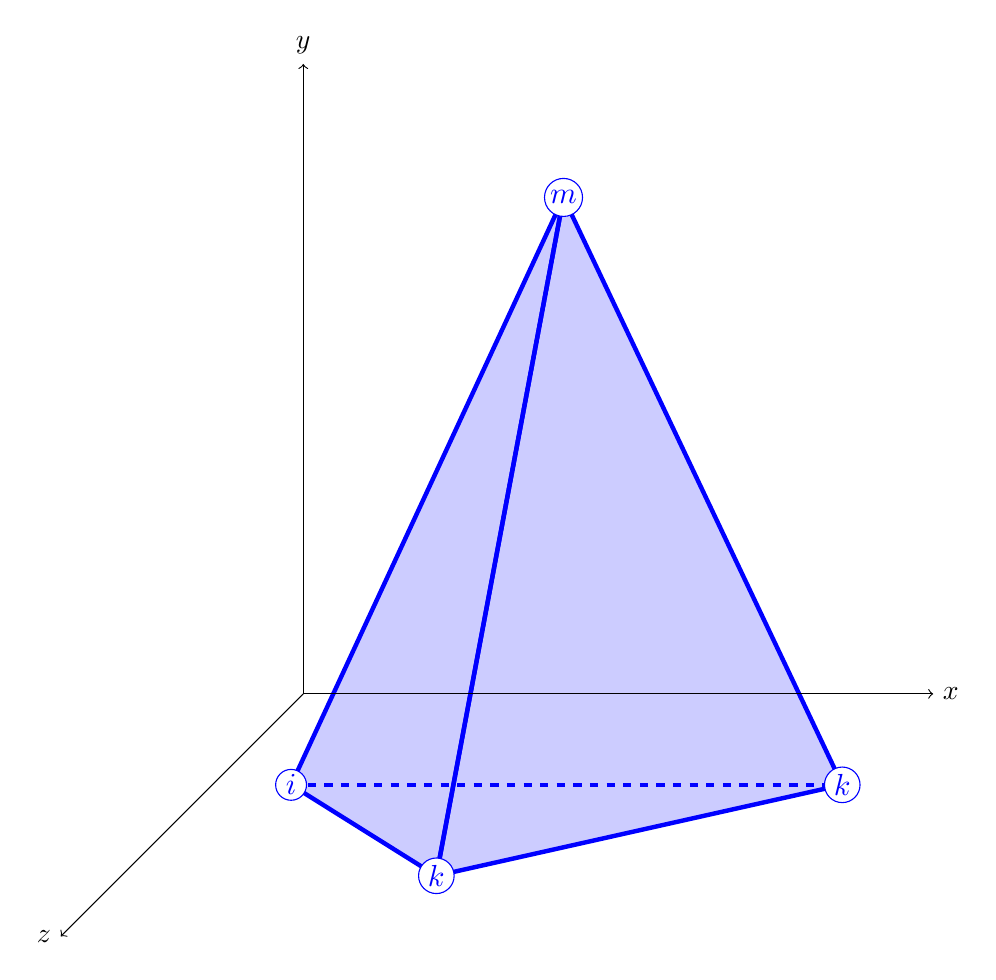
\begin{tikzpicture}
            \coordinate (i) at (1,0,3);
            \coordinate (j) at (4,0,6);
            \coordinate (k) at (8,0,3);
            \coordinate (m) at (6,9,7);
            
            \draw[blue, ultra thick, fill=blue, fill opacity = 0.2] 
                (j) 
                -- (m) -- (k)  
                -- cycle;
            \draw[blue, ultra thick, fill=blue, fill opacity = 0.2] 
            (i) -- (m) -- (j) -- cycle;
            \draw [->] (0,0,0) -- (8,0,0) node[anchor = west] {$x$};
            \draw [->] (0,0,0) -- (0,8,0) node[anchor = south] {$y$};
            \draw [->] (0,0,0) -- (0,0,8) node[anchor = east] {$z$};
            \draw[dashed, blue, ultra thick] (i) -- (k);
            \draw (i) node[blue, circle, draw, inner sep=1pt, fill=white, thin, scale = 1.1, fill opacity = 1] {$i$};
            \draw (j) node[blue, circle, draw, inner sep=1pt, fill=white, thin, scale = 1.1, fill opacity = 1] {$k$};
            \draw (k) node[blue, circle, draw, inner sep=1pt, fill=white, thin, scale = 1.1, fill opacity = 1] {$k$};
            \draw (m) node[blue, circle, draw, inner sep=1pt, fill=white, thin, scale = 1.1, fill opacity = 1] {$m$};
    \end{tikzpicture}
    \fonte{\me (2022)}
\end{figure}

Como já mencionado, a função de campo tratada aqui é o deslocamento sobre o sólido. Para cada elemento discretizado, essa função é interpolada por um polinômio, definido pelo valor do próprio campo nos nós do elemento. Em um elemento tetraédico, como o da figura \ref{fig:tetraedro}, há quatro nós ($i$, $j$, $k$ e $m$), e em cada um o campo de deslocamento tem três componentes. Essa liberdade do deslocamento que o campo tem nos nós é chamada de grau de liberdade. As funções de deslocamento, expressão \ref{eq:funcao_deslocamento}, como ditas anteriormes, são defnidas como lineares, o que garate a compatibilidade entre cada elemento, fazendo com que não existam desconitnuidades no campo de deslocamentos de acordo com \citeshort{Logan}. A função $\varphi$, portanto, pode ser decomposta em termos de suas variáveis da seguinte forma:

\begin{equation} \label{eq:linear}
    \mathbf{\varphi} = 
    \begin{Bmatrix}
        u(x,y,z) \\ v(x,y,z) \\ w(x,y,z)
    \end{Bmatrix} 
    = \begin{Bmatrix}
        a_1 + a_2 x + a_3 y + a_4 z\\
        b_1 + b_2 x + b_3 y + b_4 z\\
        c_1 + c_2 x + c_3 y + c_4 z\\
    \end{Bmatrix}
\end{equation}

Para encotrar esses fatores, basta aplicar as funções em cada nó.

\begin{equation}
    \begin{cases}
        u_i = a_1 + a_2 x_i + a_3 y_i + a_4 z_i \\
        u_j = a_1 + a_2 x_j + a_3 y_j + a_4 z_j \\
        u_k = a_1 + a_2 x_k + a_3 y_k + a_4 z_k \\
        u_m = a_1 + a_2 x_m + a_3 y_m + a_4 z_i
    \end{cases}
\end{equation}

Esse sistema pode ser rearranjado na seguinte forma matricial:

\begin{equation}
    \{\mathbf{u}\} = \begin{Bmatrix}
        u_i \\
        u_j \\
        u_k \\
        u_m
    \end{Bmatrix} = 
    \begin{bmatrix}
        1 & x_i & y_i & z_i \\
        1 & x_j & y_j & z_j \\
        1 & x_k & y_k & z_k \\
        1 & x_m & y_m & z_m \\
    \end{bmatrix}
    \begin{bmatrix}
        a_1 \\ a_2 \\ a_3 \\ a_4
    \end{bmatrix} 
\end{equation}

Portanto,

\begin{equation}
    \begin{bmatrix}
        a_1 \\ a_2 \\ a_3 \\ a_4
    \end{bmatrix}
    = \begin{bmatrix}
        1 & x_i & y_i & z_i \\
        1 & x_j & y_j & z_j \\
        1 & x_k & y_k & z_k \\
        1 & x_m & y_m & z_m \\
    \end{bmatrix}^{-1} \{\mathbf{u}\}
\end{equation}

O mesmo procedimento pode ser aplicado às outras funções de deslocamento ($v$ e $w$).




